\documentclass{standalone}
\usepackage{tikz}
\usetikzlibrary{patterns, positioning}
\usepackage[sfdefault]{ClearSans} %% option 'sfdefault' activates Clear Sans as the default text font
\usepackage[T1]{fontenc}

\begin{document}
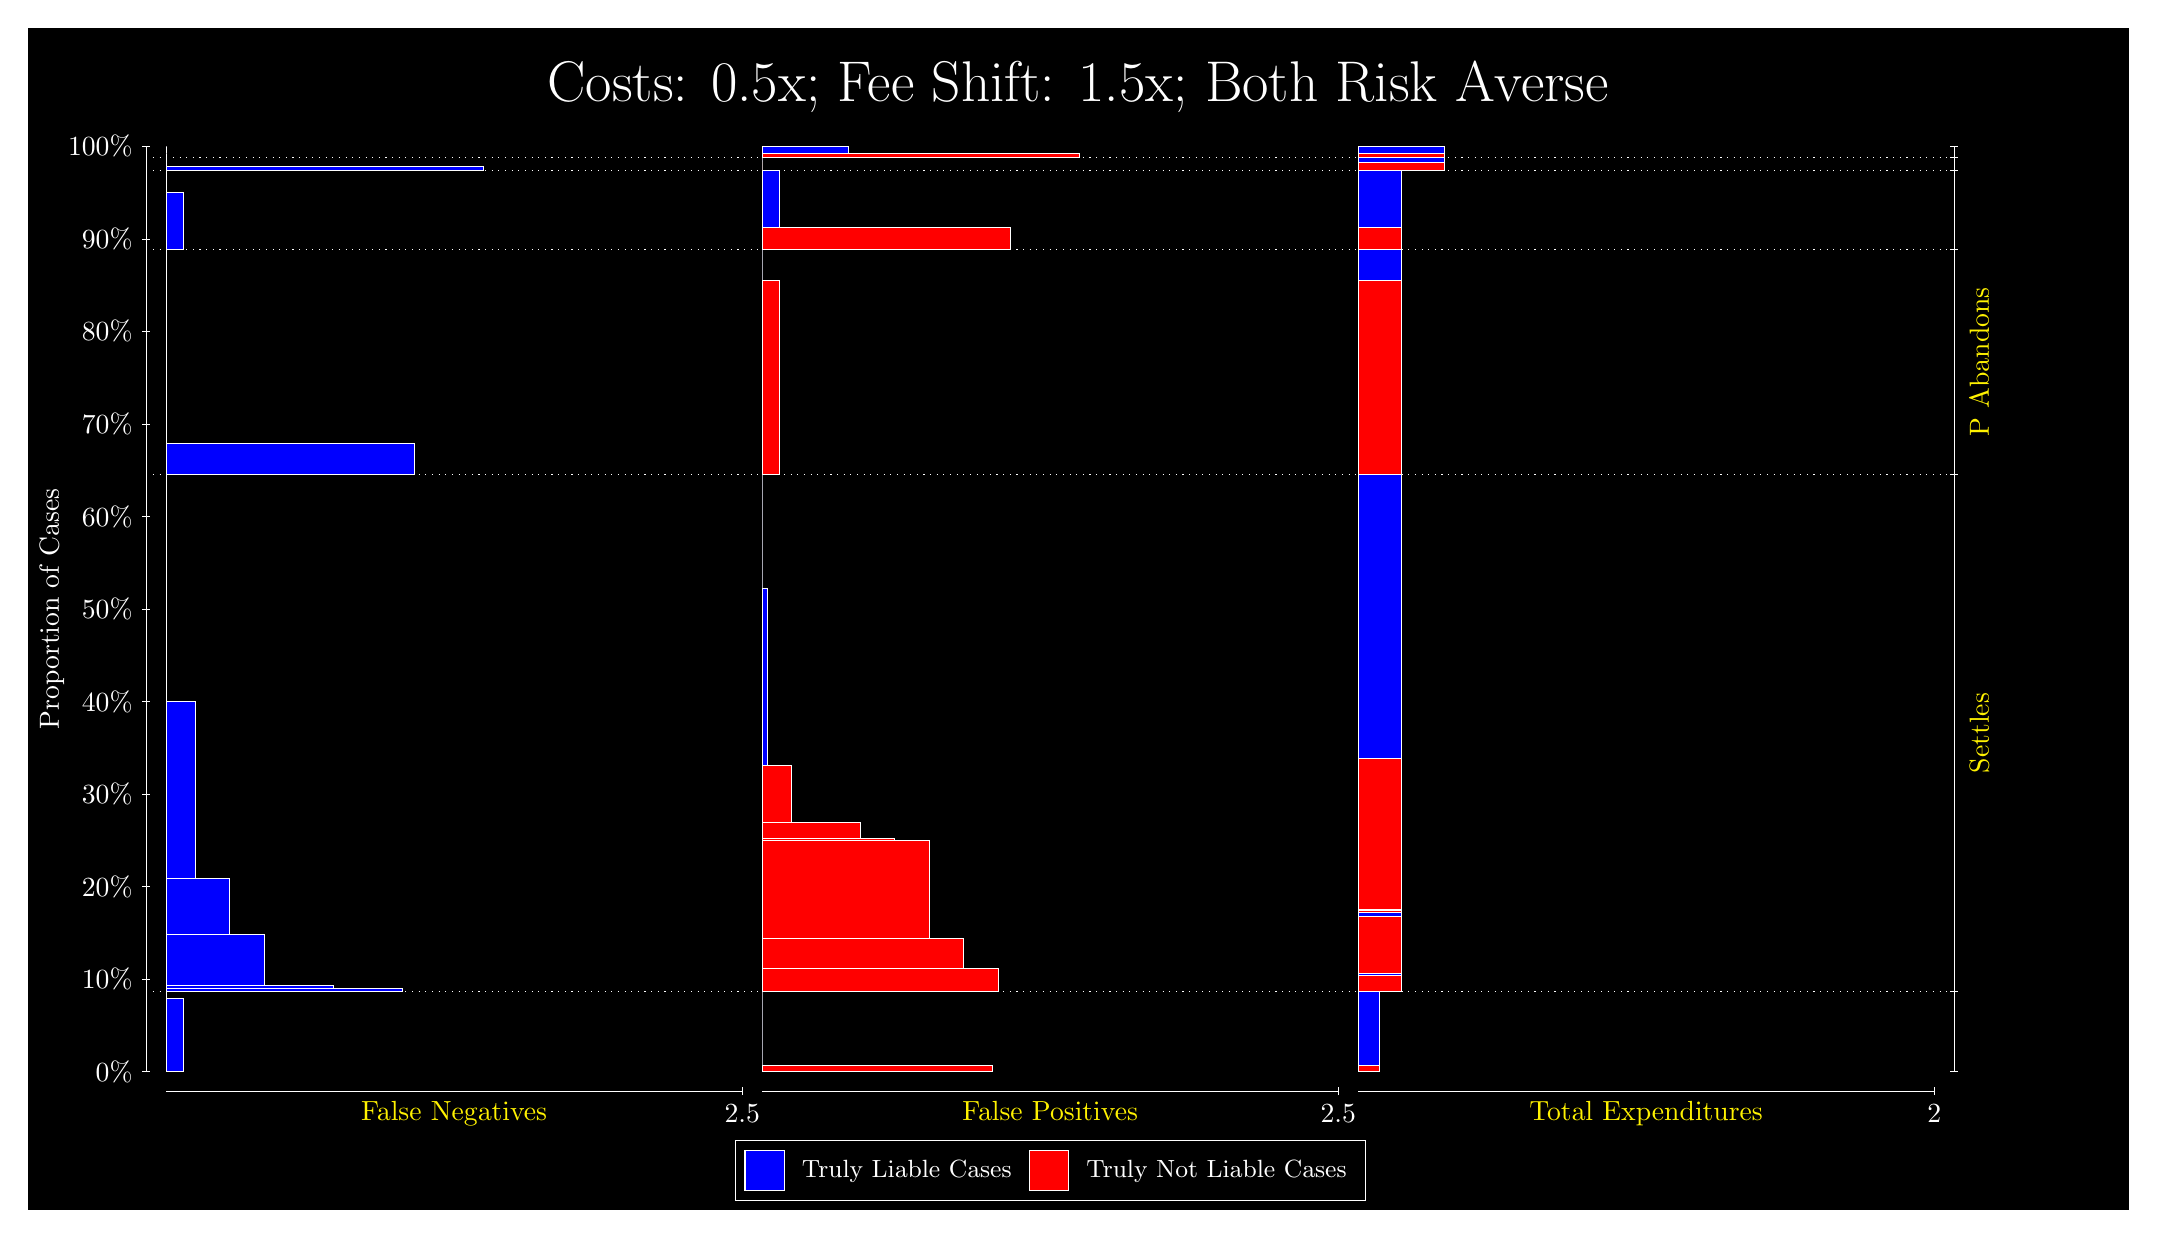
\begin{tikzpicture}
\draw[fill=black] (0,0) rectangle (26.667,15);
\draw[text=white] (0,13.5) rectangle (26.667,15) node[midway] {\huge Costs: 0.5x; Fee Shift: 1.5x; Both Risk Averse};
\draw[white, very thin] (1.5,1.75) -- (1.5,13.5);
\node[rotate=90, text=white, anchor=center] at (0.3, 7.625) {Proportion of Cases};
\draw[white, very thin] (1.45,1.75) -- (1.55,1.75);
\node[text=white, anchor=east] at (1.45, 1.75) {0\%};
\draw[white, very thin] (1.45,2.925) -- (1.55,2.925);
\node[text=white, anchor=east] at (1.45, 2.925) {10\%};
\draw[white, very thin] (1.45,4.1) -- (1.55,4.1);
\node[text=white, anchor=east] at (1.45, 4.1) {20\%};
\draw[white, very thin] (1.45,5.275) -- (1.55,5.275);
\node[text=white, anchor=east] at (1.45, 5.275) {30\%};
\draw[white, very thin] (1.45,6.45) -- (1.55,6.45);
\node[text=white, anchor=east] at (1.45, 6.45) {40\%};
\draw[white, very thin] (1.45,7.625) -- (1.55,7.625);
\node[text=white, anchor=east] at (1.45, 7.625) {50\%};
\draw[white, very thin] (1.45,8.8) -- (1.55,8.8);
\node[text=white, anchor=east] at (1.45, 8.8) {60\%};
\draw[white, very thin] (1.45,9.975) -- (1.55,9.975);
\node[text=white, anchor=east] at (1.45, 9.975) {70\%};
\draw[white, very thin] (1.45,11.15) -- (1.55,11.15);
\node[text=white, anchor=east] at (1.45, 11.15) {80\%};
\draw[white, very thin] (1.45,12.325) -- (1.55,12.325);
\node[text=white, anchor=east] at (1.45, 12.325) {90\%};
\draw[white, very thin] (1.45,13.5) -- (1.55,13.5);
\node[text=white, anchor=east] at (1.45, 13.5) {100\%};

\draw[white, very thin] (24.457,1.75) -- (24.457,13.5);
\draw[white, very thin] (24.407,1.75) -- (24.507,1.75);
\node[anchor=west] at (24.407, 1.75) {};
\draw[white, very thin] (24.407,2.7635) -- (24.507,2.7635);
\node[anchor=west] at (24.407, 2.7635) {};
\draw[white, very thin] (24.407,9.3334) -- (24.507,9.3334);
\node[anchor=west] at (24.407, 9.3334) {};
\draw[white, very thin] (24.407,12.194) -- (24.507,12.194);
\node[anchor=west] at (24.407, 12.194) {};
\draw[white, very thin] (24.407,13.192) -- (24.507,13.192);
\node[anchor=west] at (24.407, 13.192) {};
\draw[white, very thin] (24.407,13.357) -- (24.507,13.357);
\node[anchor=west] at (24.407, 13.357) {};
\draw[white, very thin] (24.407,13.5) -- (24.507,13.5);
\node[anchor=west] at (24.407, 13.5) {};

\draw[white, very thin, fill=blue] (1.75,1.75) rectangle (1.9696,2.6814);
\draw[white, very thin, fill=red] (1.75,2.6814) rectangle (1.75,2.7635);
\draw[white, very thin, fill=blue] (1.75,2.7635) rectangle (4.7507,2.8109);
\draw[white, very thin, fill=blue] (1.75,2.8109) rectangle (3.8725,2.8391);
\draw[white, very thin, fill=blue] (1.75,2.8391) rectangle (3.4333,2.8486);
\draw[white, very thin, fill=blue] (1.75,2.8486) rectangle (2.9942,3.4913);
\draw[white, very thin, fill=blue] (1.75,3.4913) rectangle (2.5551,4.2055);
\draw[white, very thin, fill=blue] (1.75,4.2055) rectangle (2.1159,6.4532);
\draw[white, very thin, fill=red] (1.75,6.4532) rectangle (1.75,9.3334);
\draw[white, very thin, fill=blue] (1.75,9.3334) rectangle (4.8971,9.724);
\draw[white, very thin, fill=red] (1.75,9.724) rectangle (1.75,12.194);
\draw[white, very thin, fill=blue] (1.75,12.194) rectangle (1.9696,12.915);
\draw[white, very thin, fill=red] (1.75,12.915) rectangle (1.75,13.192);
\draw[white, very thin, fill=blue] (1.75,13.192) rectangle (5.7754,13.245);
\draw[white, very thin, fill=red] (1.75,13.245) rectangle (1.75,13.357);
\draw[white, very thin, fill=red] (1.75,13.357) rectangle (1.75,13.411);
\draw[white, very thin, fill=blue] (1.75,13.411) rectangle (1.75,13.5);
\draw[white, very thin, fill=red] (9.3189,1.75) rectangle (12.246,1.832);
\draw[white, very thin, fill=blue] (9.3189,1.832) rectangle (9.3189,2.7635);
\draw[white, very thin, fill=red] (9.3189,2.7635) rectangle (12.32,3.0554);
\draw[white, very thin, fill=red] (9.3189,3.0554) rectangle (11.88,3.4447);
\draw[white, very thin, fill=red] (9.3189,3.4447) rectangle (11.441,4.6852);
\draw[white, very thin, fill=red] (9.3189,4.6852) rectangle (11.002,4.7103);
\draw[white, very thin, fill=red] (9.3189,4.7103) rectangle (10.563,4.9129);
\draw[white, very thin, fill=red] (9.3189,4.9129) rectangle (9.6848,5.6437);
\draw[white, very thin, fill=blue] (9.3189,5.6437) rectangle (9.3921,7.8914);
\draw[white, very thin, fill=blue] (9.3189,7.8914) rectangle (9.3189,9.3334);
\draw[white, very thin, fill=red] (9.3189,9.3334) rectangle (9.5384,11.804);
\draw[white, very thin, fill=blue] (9.3189,11.804) rectangle (9.3189,12.194);
\draw[white, very thin, fill=red] (9.3189,12.194) rectangle (12.466,12.471);
\draw[white, very thin, fill=blue] (9.3189,12.471) rectangle (9.5384,13.192);
\draw[white, very thin, fill=red] (9.3189,13.192) rectangle (9.3189,13.303);
\draw[white, very thin, fill=blue] (9.3189,13.303) rectangle (9.3189,13.357);
\draw[white, very thin, fill=red] (9.3189,13.357) rectangle (13.344,13.411);
\draw[white, very thin, fill=blue] (9.3189,13.411) rectangle (10.417,13.5);
\draw[white, very thin, fill=red] (16.888,1.75) rectangle (17.162,1.832);
\draw[white, very thin, fill=blue] (16.888,1.832) rectangle (17.162,2.7635);
\draw[white, very thin, fill=red] (16.888,2.7635) rectangle (17.437,2.9662);
\draw[white, very thin, fill=blue] (16.888,2.9662) rectangle (17.437,2.9945);
\draw[white, very thin, fill=red] (16.888,2.9945) rectangle (17.437,3.7252);
\draw[white, very thin, fill=blue] (16.888,3.7252) rectangle (17.437,3.7726);
\draw[white, very thin, fill=red] (16.888,3.7726) rectangle (17.437,3.7976);
\draw[white, very thin, fill=blue] (16.888,3.7976) rectangle (17.437,3.8071);
\draw[white, very thin, fill=red] (16.888,3.8071) rectangle (17.437,5.7287);
\draw[white, very thin, fill=blue] (16.888,5.7287) rectangle (17.437,9.3334);
\draw[white, very thin, fill=red] (16.888,9.3334) rectangle (17.437,11.804);
\draw[white, very thin, fill=blue] (16.888,11.804) rectangle (17.437,12.194);
\draw[white, very thin, fill=red] (16.888,12.194) rectangle (17.437,12.471);
\draw[white, very thin, fill=blue] (16.888,12.471) rectangle (17.437,13.192);
\draw[white, very thin, fill=red] (16.888,13.192) rectangle (17.986,13.303);
\draw[white, very thin, fill=blue] (16.888,13.303) rectangle (17.986,13.357);
\draw[white, very thin, fill=red] (16.888,13.357) rectangle (17.986,13.411);
\draw[white, very thin, fill=blue] (16.888,13.411) rectangle (17.986,13.5);
\draw[white, dotted] (1.5,2.7635) -- (24.457,2.7635);
\draw[white, dotted] (1.5,9.3334) -- (24.457,9.3334);
\draw[white, dotted] (1.5,12.194) -- (24.457,12.194);
\draw[white, dotted] (1.5,13.192) -- (24.457,13.192);
\draw[white, dotted] (1.5,13.357) -- (24.457,13.357);
\draw[white, very thin] (1.75,1.5) -- (9.0689,1.5);
\node[text=yellow, anchor=north] at (5.4094, 1.5) {False Negatives};
\draw[white, very thin] (9.0689,1.45) -- (9.0689,1.55);
\node[text=white, anchor=north] at (9.0689, 1.45) {2.5};

\draw[white, very thin] (9.3189,1.5) -- (16.638,1.5);
\node[text=yellow, anchor=north] at (12.978, 1.5) {False Positives};
\draw[white, very thin] (16.638,1.45) -- (16.638,1.55);
\node[text=white, anchor=north] at (16.638, 1.45) {2.5};

\draw[white, very thin] (16.888,1.5) -- (24.207,1.5);
\node[text=yellow, anchor=north] at (20.547, 1.5) {Total Expenditures};
\draw[white, very thin] (24.207,1.45) -- (24.207,1.55);
\node[text=white, anchor=north] at (24.207, 1.45) {2};


\node[text=yellow, centered, rotate=90] at (24.777, 6.0484) {Settles};
\node[text=yellow, centered, rotate=90] at (24.777, 10.764) {P Abandons};




\draw (12.978300999999998,1.5) node[draw=none] (baseCoordinate) {};
\begin{scope}[align=center]
        \matrix[scale=0.5, draw=white, below=0.5cm of baseCoordinate, nodes={draw}, column sep=0.1cm]{
            \node[rectangle, draw, minimum width=0.5cm, minimum height=0.5cm, fill=blue] {}; &
            \node[draw=none, font=\small, text=white] (B) {Truly Liable Cases}; &
            \node[rectangle, draw, minimum width=0.5cm, minimum height=0.5cm, fill=red] {}; &
            \node[draw=none, font=\small, text=white] (B) {Truly Not Liable Cases}; \\
            };
\end{scope}

\end{tikzpicture}
\end{document}